\documentclass{article}

% Numbered citations keep the four-page main text compact.
\PassOptionsToPackage{numbers,compress,sort}{natbib}
\usepackage[preprint]{neurips_2025}

\usepackage[utf8]{inputenc}
\usepackage[T1]{fontenc}
\usepackage{hyperref}
\usepackage{url}
\usepackage{booktabs}
\usepackage{amsfonts}
\usepackage{amsmath}
\usepackage{amssymb}
\usepackage{nicefrac}
\usepackage{microtype}
\usepackage{xcolor}
\usepackage{graphicx}
\usepackage{array}
\usepackage{makecell}
\usepackage{pifont}
\usepackage[font=small,labelfont=bf,skip=3pt]{caption}
\usepackage[shortlabels]{enumitem}
\usepackage{placeins}
\usepackage{listings}
\lstset{basicstyle=\ttfamily\scriptsize,columns=fullflexible,keepspaces=true,frame=tb,framesep=3pt,
  showstringspaces=false,upquote=true,aboveskip=6pt,belowskip=4pt,keywordstyle=\ttfamily,
  commentstyle=\upshape\color{black!60},stringstyle=\upshape\color{black!70}}

% Figures: the repository's figures/ folder and the figures drawn for this paper (figures_own/).
\graphicspath{{../figures/}{figures_own/}}
\hypersetup{colorlinks=true,linkcolor=black,citecolor=blue!50!black,urlcolor=blue!50!black}

\newcommand{\cmark}{\ding{51}}
\newcommand{\xmark}{\ding{55}}
\newcommand{\up}{$^{\uparrow}$}
\newcommand{\dn}{$^{\downarrow}$}
% Panel label set above a figure panel of the given width (the figures themselves carry no letters).
\newcommand{\plabel}[3]{\makebox[#1][l]{\small\textbf{#2}~#3}}
% Numbered run-in subsection heading (same look as \paragraph of the style file, with a number).
\newcommand{\rsub}[1]{\refstepcounter{subsection}\paragraph{\thesubsection~~#1}}

\title{Is It the Model or the Reading?\\A Fast-Weight View of ViT Attention Maps}

\author{Hongbo Huang\\Student ID: 50026755}

\begin{document}

\maketitle

\begin{abstract}
Deep-layer attention maps of vision transformers (ViTs) often look poor: scattered, with much score on a few background patches. The usual remedy changes the model; we ask how much of the problem lies in how the map is read. A long-standing fast-weight view treats an attention head as a two-layer network with the tokens as hidden units. We state three premises of reading these units, measure a diagnostic for each on DeiT-S, DeiT-B and DINO ViT-S, and test a correction against a matched control. Our pre-registered prediction that the three corrections together improve deep-layer maps holds in one of four cases. Singly, contribution weighting, in practice the value-norm weighting of Kobayashi et al.\ and Zhu et al., improves localisation and human alignment in the two models its diagnostic flags (object enrichment $+0.038$ and $+0.065$) and nothing in the third, while relocating scores with a position probe harms every map, so this diagnostic may not measure its premise. On DeiT-S, two model-side changes do not exceed our margin. Part of what makes deep maps look poor is how we read them.
\end{abstract}

% =====================================================================================================
\section{Introduction}

Attention maps are widely used to show what a vision transformer (ViT)~\citep{dosovitskiy2021} looks at~\citep{caron2021,abnar2020,chefer2021generic}. In deep layers they often look poor: the score is scattered, much of it on a few background patches~\citep{darcet2024} (Fig.~\ref{fig:lens}b). The usual remedy changes the model: register tokens absorb the stray attention~\citep{darcet2024,jiang2025}. We ask instead: \emph{how much of the problem lies in how the map is read?}

\begin{figure}[!h]
\centering
\plabel{1.95in}{(a)}{The lens}\hspace{0.3in}\plabel{2.85in}{(b)}{Example maps (DeiT-S, layers 9--12)}\\[2pt]
\raisebox{-0.5\height}{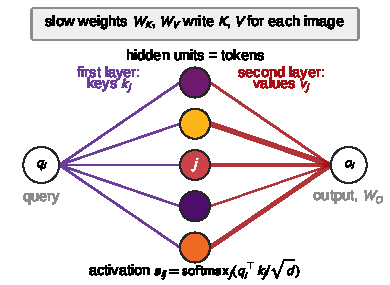
\includegraphics[width=1.95in]{schematic_fast_weight_network}}\hspace{0.3in}\raisebox{-0.5\height}{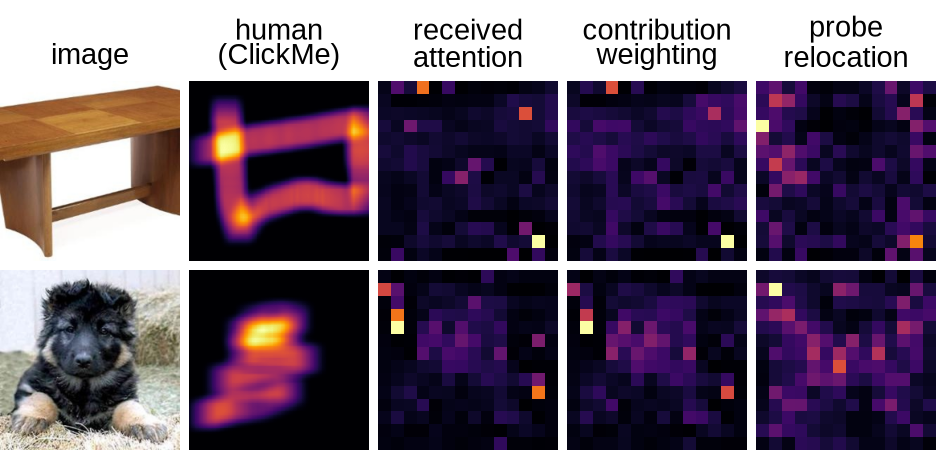
\includegraphics[width=2.85in]{example_maps}}
\caption{(a) For one image, an attention head is a two-layer network: slow weights $W_K, W_V$ write its weights (keys, values); tokens are hidden units. (b) Two randomly drawn ClickMe images (min--max normalised).}
\label{fig:lens}
\end{figure}

A map is a model plus a reading rule, and the rule is rarely examined. We view an attention head as a two-layer network that is written anew for each image and has the tokens as its hidden units (Fig.~\ref{fig:lens}a), a long-standing fast-weight view. The common \emph{received-attention} map then reads these hidden units, which rests on three premises: activations are specific to the image, unit $j$ still stands for patch $j$, and a large activation is a large contribution. On DeiT-S, DeiT-B~\citep{touvron2021} and DINO ViT-S~\citep{caron2021}, we measure a diagnostic for each premise per layer, test a correction against a matched control, and compare the outcomes with pre-registered predictions. Our contributions are:
\begin{enumerate}[nosep,leftmargin=1.7em,label=(\arabic*)]
\item \textbf{Premises.} Three testable premises of the attention-map reading, each with a diagnostic.
\item \textbf{A reading-side repair.} Value-norm weighting~\citep{kobayashi2020,zhu2024} improves localisation and human alignment in the two models that its diagnostic flags, and nothing in the third.
\item \textbf{Negative results.} The registered prediction that the corrections add up holds in one of four cells, and probe relocation harms every map: the probe does not measure the location premise itself.
\end{enumerate}

% =====================================================================================================
\section{Related work}
\label{sec:related}

\rsub{How attention maps are read and scored.} Whether attention explains predictions is debated~\citep{jain2019,wiegreffe2019}. Later readings add layers~\citep{abnar2020}, relevance propagation~\citep{chefer2021}, gradients~\citep{chefer2021generic}, vector norms~\citep{kobayashi2020,zhu2024} or statistical filtering~\citep{ayyar2025}. Scoring has traps: plausible maps can ignore the model~\citep{adebayo2018}, deletion depends on the occlusion strategy~\citep{bluecher2024}, and random CNNs give centred saliency~\citep{kuang2026} (largely absent in ViTs). Most compare readings by \emph{results}; \citet{kobayashi2020} question our third premise.

\rsub{Why deep ViT maps degrade.} Deep maps put much attention on high-norm background tokens, which registers absorb~\citep{darcet2024,jiang2025}; such tokens resemble heads that learn to do nothing~\citep{bondarenko2023}, and supervision shapes attention~\citep{walmer2023}. Tokens also mix: in language models their identity is largely kept but fades~\citep{brunner2020}, and in CLS-trained ViTs last-layer tokens still resemble their own input patch~\citep{raghu2021}.

\rsub{Attention as a fast-weight network.} Fast weights are weights that one network writes for another~\citep{schmidhuber1992}; linear attention is such a program~\citep{schlag2021}, and softmax attention is the update rule of a modern Hopfield memory~\citep{ramsauer2021}. This view is not ours and has mostly guided model design, as in MiTA~\citep{wen2026mita}; to our knowledge, it has not been used to test how attention maps are read.

% =====================================================================================================
\section{Method}
\label{sec:method}

\rsub{The lens.} In layer $\ell$, the normalised tokens $x_1,\dots,x_{N+1}$ (CLS and $N{=}196$ patches) enter $H$ heads. Head $h$ forms $q_i^h{=}W_Q^h x_i$, $k_j^h{=}W_K^h x_j$ and $v_j^h{=}W_V^h x_j$, and the block adds to token $i$
\begin{equation}
o_i=\sum_{h} W_O^h \sum_{j} a_{ij}^h\, v_j^h,\qquad a_{ij}^h=\operatorname{softmax}_j\!\big(q_i^{h\top} k_j^h/\sqrt{d}\big).
\label{eq:attn}
\end{equation}
For a fixed image this is a two-layer network applied to $q_i$: token $j$ is a hidden unit with input weights $k_j^h$, activation $a_{ij}^h$ and output weights $W_O^h v_j^h$. As the softmax makes units compete, the network is a guiding approximation, not an exact equivalence. \emph{Received attention} sums each unit's activation over queries and heads, $s_j=\sum_h\sum_i a_{ij}^h$, and draws it at patch $j$. As our question concerns deep layers, maps sum $s_j$ over layers 9--12 (the last third), a range set before the experiments.

\rsub{From reading units to premises.} If a head is a network, an attention map \emph{reads its hidden units}, and three lessons about reading units each give a premise (Table~\ref{tab:premises}): what is there for every input says nothing about this input; what a unit stands for must be measured, not read off its index~\citep{bau2017}; and a large activation is not a large effect, because output weights count too~\citep{zhou2016}. No single premise needs the lens (the third is the point of \citet{kobayashi2020}); it gives the list and adds the location premise, which the readings of Section~\ref{sec:related} all assume. Each premise gets a diagnostic, a correction and a matched control that changes the map alike without the premise's information. Diagnostics are proxies, not the premises themselves, and $c_j$ measures the size of a token's output, not its effect on the prediction: norms ignore cancellation between heads and all later layers. A correction counts only if it beats its control; it should help where its diagnostic flags a failure and change little elsewhere.

\begin{table}[t]
\caption{The premises, their tests, and the outcome in layers 9--12 on the centre-blind metrics (S, B, D: DeiT-S, DeiT-B, DINO ViT-S). $^\ast$One gain, equal to its control's. $^\dagger$On B ClickMe, not beyond its control.}
\label{tab:premises}
\centering\footnotesize
\setlength{\tabcolsep}{3pt}
\renewcommand{\arraystretch}{0.92}
\begin{tabular}{@{}>{\raggedright\arraybackslash}p{1.15in}>{\raggedright\arraybackslash}p{1.06in}>{\raggedright\arraybackslash}p{1.17in}>{\raggedright\arraybackslash}p{0.89in}>{\raggedright\arraybackslash}p{0.44in}>{\raggedright\arraybackslash}p{0.36in}@{}}
\toprule
Premise & Diagnostic (a proxy) & Correction & Matched control & Flagged & Helps\\
\midrule
\textbf{Specificity:} activations are image-specific & variance explained by the mean map $\bar s$ & mean-map subtraction, $s-\bar s$ & centred Gaussian subtraction & none & none$^\ast$\\[1.5pt]
\textbf{Location:} unit $j$ still stands for patch $j$ & probe accuracy for the patch index of $x_j$ & probe relocation, $r_p{=}\sum_j s_j P(p\,|\,x_j)$ & blur of equal displacement & S, B, D & none\\[1.5pt]
\textbf{Contribution:} large activation, large effect & share of $s$ on high-norm tokens & contribution weighting, $c_j{=}\sum_{h,i} a_{ij}^h\lVert W_O^h v_j^h\rVert$ & zero the high-norm tokens & S, B & S, B$^\dagger$\\
\bottomrule
\end{tabular}
\end{table}

\rsub{Metrics.} A centre prior can inflate scores: in our data, a centred Gaussian has a Spearman correlation of 0.41 with human ClickMe maps. Two metrics are therefore centre-blind: \emph{same-ring object enrichment}, the object rate (ImageNet-S masks~\citep{gao2023}) of the top-scoring patches minus that of all patches equally far from the centre, and \emph{image-specific ClickMe alignment}~\citep{linsley2019,fel2022}, the Spearman correlation with the image's own human map minus that with another image's. \emph{Deletion faithfulness}~\citep{bluecher2024} is not centre-blind. A paired difference is \emph{higher} or \emph{lower} only if its 95\% bootstrap interval excludes zero and it exceeds a margin (0.02; 0.05 for deletion); else it is \emph{comparable}.

% =====================================================================================================
\section{Experiments}
\label{sec:exp}

\rsub{Setup and registered predictions.} We use frozen DeiT-S and DeiT-B~\citep{touvron2021} (supervised) and DINO ViT-S/16~\citep{caron2021}; the model-side changes are a test-time register~\citep{jiang2025} and the top-$k$-attention checkpoint of MiTA~\citep{wen2026mita}, both for DeiT-S. Data: 5,000 ImageNet~\citep{deng2009} and 12,419 ImageNet-S images, 17,408 ClickMe maps and 4,000 held-out images (App.~\ref{app:setup}). Before the experiments we fixed metrics, margins and comparisons and registered three predictions (App.~\ref{app:setup}). \textbf{R1:} where a diagnostic shows no failure, the correction leaves the map comparable (contribution weighting in DINO ViT-S; relocation at layers 1--4). \textbf{R2:} the three corrections together are higher than received attention in the four supervised centre-blind cells. \textbf{R3:} neither model-side change is higher than DeiT-S. For single corrections against their controls we fixed no direction. Other analyses are \emph{post hoc}.

\begin{figure}[t]
\centering
\plabel{1.3975in}{(a)}{Specificity}\plabel{1.3975in}{(b)}{Location}\plabel{1.3975in}{(c)}{Contribution}\plabel{1.3075in}{(d)}{Map quality}\\[1pt]
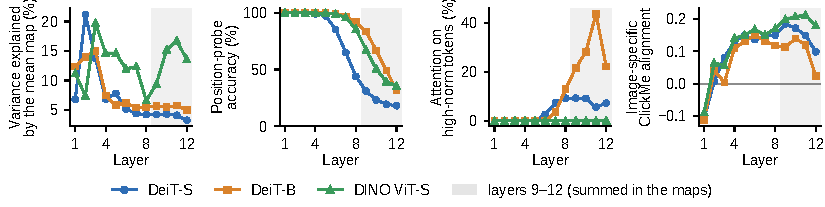
\includegraphics[width=5.5in]{diagnosis}
\caption{Per layer: (a) map variance explained by the mean map; (b) position-probe accuracy; (c) attention on high-norm tokens; (d) image-specific ClickMe alignment of single-layer maps. Bands: 95\% intervals.}
\label{fig:diag}
\end{figure}

\rsub{Attention marks the units the model uses.} If, in every head and layer, each query reads only the $k{=}16$ units (of 196) that score highest for its region, the models keep 72\%, 83\% and 61\% of their top-1 predictions, against 9\%, 30\% and 4\% for random units, also for other $k$ (App.~\ref{app:more}).

\rsub{Two diagnostics flag deep layers (Fig.~\ref{fig:diag}).} \emph{Specificity} shows no failure: in layers 6--12 the mean map explains 3--6\% of a map's spatial variance in the supervised models and at most 17\% in DINO ViT-S, and in layers 9--12 it is 82--98\% radial. The \emph{location} diagnostic weakens in all models: probe accuracy falls from nearly 100\% in layers 1--5 to 18\%, 32\% and 36\% at layer 12 (chance: 0.5\%), although 45\%, 66\% and 81\% of its probability lies in the $3{\times}3$ neighbourhood of the true patch. The \emph{contribution} diagnostic flags only the supervised models: high-norm tokens (norm over three times the image median) get up to 44\% of the attention in DeiT-B and 9\% in DeiT-S but none in DINO ViT-S~\citep{darcet2024}, with value vectors 0.29 and 0.23 times as long as other patches'.

\begin{table}[t]
\caption{Layers 9--12, controls indented: enrichment (Enr.), ClickMe (Click.), deletion (Del.). $^{\uparrow}$/$^{\downarrow}$: higher/lower than received attention (model-side: than DeiT-S). GAE~\citep{chefer2021generic} also uses gradients; it has no significance test.}
\label{tab:main}
\centering\footnotesize
\setlength{\tabcolsep}{2.6pt}
\renewcommand{\arraystretch}{0.9}
% Table 1: made by make/make_main_table.py from results/table1_long.csv, correct_tests.csv and variants.csv.
\begin{tabular}{@{}l@{\hspace{4pt}}ccc@{\hspace{7pt}}ccc@{\hspace{7pt}}ccc@{}}
\toprule
 & \multicolumn{3}{c}{DeiT-S} & \multicolumn{3}{c}{DeiT-B} & \multicolumn{3}{c}{DINO ViT-S}\\
\cmidrule(r{6pt}){2-4}\cmidrule(r{6pt}){5-7}\cmidrule{8-10}
Reading & Enr. & Click. & Del. & Enr. & Click. & Del. & Enr. & Click. & Del.\\
\midrule
Received attention & 0.140 & 0.157 & 0.236 & 0.080 & 0.107 & 0.169 & 0.199 & 0.208 & 0.285 \\
Contribution weighting & 0.178\up & 0.190\up & 0.253 & 0.146\up & 0.165\up & 0.198 & 0.196 & 0.207 & 0.285 \\
\quad zero high-norm tokens & 0.152 & 0.168 & 0.241 & 0.121\up & 0.148\up & 0.186 & 0.199 & 0.208 & 0.285 \\
Mean-map subtraction & 0.138 & 0.165 & 0.208 & 0.077 & 0.087\dn & 0.144 & 0.201 & 0.252\up & 0.233\dn \\
\quad centre-Gaussian subtraction & 0.133 & 0.168 & 0.167\dn & 0.056\dn & 0.062\dn & 0.024\dn & 0.200 & 0.253\up & 0.232\dn \\
Probe relocation & 0.041\dn & 0.084\dn & 0.076\dn & 0.027\dn & 0.050\dn & 0.051\dn & 0.084\dn & 0.143\dn & 0.141\dn \\
\quad matched blur & 0.095\dn & 0.152 & 0.181\dn & $-$0.008\dn & 0.068\dn & 0.097\dn & 0.189 & 0.226 & 0.287 \\
All three corrections & 0.059\dn & 0.123\dn & 0.076\dn & 0.079 & 0.137\up & 0.085\dn & 0.088\dn & 0.177\dn & 0.090\dn \\
\midrule
+ test-time register & 0.152 & 0.169 & 0.236 & -- & -- & -- & -- & -- & -- \\
Top-$k$ training (MiTA) & 0.100\dn & 0.115\dn & -- & -- & -- & -- & -- & -- & -- \\
GAE (reference) & 0.204 & 0.234 & 0.345 & 0.196 & 0.213 & 0.308 & 0.221 & 0.234 & 0.418 \\
\bottomrule
\end{tabular}

\end{table}

\rsub{Only contribution weighting improves the map (Table~\ref{tab:main}).} \emph{R1 holds:} in DINO ViT-S, contribution weighting leaves all metrics comparable, and relocation at layers 1--4 changes the centre-blind metrics by at most 0.004. \emph{R2 holds in one of four cells} (DeiT-B ClickMe). \emph{Contribution weighting} is higher on both centre-blind metrics in DeiT-S and DeiT-B ($+0.033$ to $+0.065$), beating its control except on DeiT-B ClickMe, and comparable on deletion: localisation and human alignment improve, deletion faithfulness stays within the margin. In DeiT-B, zeroing the high-norm tokens gives $+0.040$ of the $+0.065$ on enrichment. Post hoc, it beats the same weights shuffled within each head in all four cells ($+0.035$ to $+0.073$), gains more on images with more attention on high-norm tokens, and is matched by weighting with $\lVert v_j\rVert$ alone (App.~\ref{app:more}): in practice it is value-norm weighting~\citep{kobayashi2020,zhu2024}. At layer 12 it recovers 31--62\% of the drop in map quality (Fig.~\ref{fig:diag}d). \emph{Mean-map subtraction} gains only on DINO ViT-S ClickMe, as much as its control. \emph{Probe relocation} is lower in all nine cells, and in DeiT-S and DINO ViT-S lower even than its matched blur. \emph{R3 holds:} the register gains $+0.012$ and $+0.013$, below the margin; the top-$k$ checkpoint is lower, but differs from DeiT-S in training and preprocessing, so the comparison is uncontrolled.

\rsub{Does the diagnosis tell where a correction helps (Table~\ref{tab:premises}, right)?} We registered no direction for single corrections, so this reading is post hoc. For \emph{contribution} it is consistent: the correction helps in the two flagged models and changes nothing in DINO ViT-S. For \emph{specificity} there was little to correct, and nothing is gained beyond the control. For \emph{location} it is not: the diagnostic weakens in every model, yet relocation harms every map. Four explanations, such as far probe errors or a weak probe, found no support (post hoc; App.~\ref{app:reloc}). A fifth, untested, concerns the diagnostic: the probe measures whether a token's patch index can be decoded, not where its content comes from. A token may lose its position code and still carry patch $j$ (cf.~\citep{raghu2021}); the index then stays the better guide. Diagnosis and correction agree for one premise in three models, which does not establish the idea.

% =====================================================================================================
\section{Discussion}
\label{sec:discussion}

\rsub{Interpretation.} \emph{Activation is not effect:} high-norm tokens draw attention but have short value vectors, like heads that do nothing~\citep{bondarenko2023}; weighting by output-weight norms partly repairs the map without changing the model. \emph{A weaker position code is not a moved token:} to test the location premise itself, one must measure which input patches a token depends on.

\rsub{Limitations.} We study three classifiers at S/B scale, each trained once, and only received attention; CLS attention, larger or register-trained models and model-side changes beyond DeiT-S are untested. Diagnostics are proxies, and the high-norm threshold was not varied. ClickMe images were very likely training data. Gains are modest, hard to see in one image (Fig.~\ref{fig:lens}b), and below GAE's.

\rsub{Ethical considerations.} We use public data and checkpoints; the images include people and known biases. An attention map, corrected or not, is only partial evidence about a model.

% =====================================================================================================
\section{Conclusion}
\label{sec:conclusion}

For ViT attention maps, the fast-weight view gives three premises to check: correcting the contribution premise partly repairs deep maps in the models that its diagnostic flags, the location correction fails, and the corrections do not add up. We tested only ViT attention maps, but the same question applies to any method that maps internal values to input positions. Future work should test the location premise with token-to-input attribution and cover larger and register-trained models and CLS attention. As a broader impact, premise tests need no retraining and can keep users from over-trusting a map.

{\small
\bibliographystyle{plainnat}
\bibliography{references}
}

\clearpage
\appendix
% =====================================================================================================
% Appendix: experimental details (A), additional results (B), analysis of probe relocation (C),
% example maps (D), exploratory tests (E) and key code (F).
% =====================================================================================================

\counterwithin{figure}{section}
\counterwithin{table}{section}
\captionsetup{skip=5pt}
\raggedbottom

\section{Experimental details}
\label{app:setup}

\paragraph{Models.} All models are frozen ViTs with $16{\times}16$ patches on $224{\times}224$ inputs. The three baseline backbones come from timm~\citep{wightman2019}. \emph{DeiT-S and DeiT-B}~\citep{touvron2021}: \texttt{deit\_small\_patch16\_224.fb\_in1k} and \texttt{deit\_base\_patch16\_224.fb\_in1k} (resize to 248, centre crop 224: a crop ratio of 0.9). \emph{DINO ViT-S/16}~\citep{caron2021}: \texttt{vit\_small\_patch16\_224.dino} with the official DINO linear head (resize to 256, centre crop 224: a crop ratio of 0.875). \emph{DeiT-S with a test-time register}~\citep{jiang2025}: the activations of eight feed-forward units in layers 4 and 5 are moved to one added register token, which is left out of every map, like CLS. The units were selected on 500 ImageNet-S images, where they reduce the number of high-norm patch tokens (counted per layer) by 92.75\% and keep 99.0\% of the predictions; on the other 11,919 images the reduction is 91.5\%, and ImageNet accuracy stays at 79.8\%. For DeiT-B the same search found no such units (44.9\% reduction with 32 units), so we report the register for DeiT-S only. \emph{Top-$k$ training}: the DeiT-S checkpoint released with MiTA~\citep{wen2026mita} (25 summary slots, $k=25$), with its own preprocessing (crop ratio 0.875). It differs from our DeiT-S in training and preprocessing, so its row in Table~\ref{tab:main} is not a controlled comparison; its deletion score is undefined because its summary slots pool fixed regions of the full grid. Both model-side changes are tested at size S only.

\paragraph{Attention conventions.} With $x$ the output of the block's first layer norm, projections include the checkpoint's biases:
\[
q_i^h=W_Q^hx_i+b_Q^h,\quad k_j^h=W_K^hx_j+b_K^h,\quad v_j^h=W_V^hx_j+b_V^h.
\]
Equation~\ref{eq:attn} includes the output bias $b_O$ and describes the attention branch before residual addition, with dropout inactive at evaluation. $W_O^h$ is the head's slice of the output projection. Value weighting assigns the per-head vector magnitudes to patches; the shared output bias is not assigned to any patch. The fixed-image two-layer representation uses the coupled softmax activation, rather than an elementwise nonlinearity.

\paragraph{Data.} \emph{Execution test}: 5,000 randomly drawn ImageNet validation images~\citep{deng2009}. \emph{ImageNet-S}~\citep{gao2023}: all 12,419 validation images with segmentation masks; stored enrichment is finite for 12,150 (12,144 for DINO). All-foreground grids score zero. Restricting enrichment to crops with both classes changed the value-weighting contrast by less than 0.002 in each model; the reported enrichment verdicts use the original eligibility rule. Deletion uses a fixed random subset of 2,000. \emph{ClickMe}~\citep{linsley2019,fel2022}: the 17,408-image validation split released with Harmonization (17 \texttt{val-*.tfrecords} shards). This split name does not identify the original ImageNet split of each image. Images are resized from $256{\times}256$ to $224{\times}224$ without cropping; heatmaps are resized to $64{\times}64$, blurred with a $10{\times}10$ Gaussian ($\sigma=10$), then resized to $224{\times}224$ (bilinear interpolation). \emph{Held-out set}: 4,000 ImageNet validation images excluded from map-quality and execution evaluation; 2,000 train probes and 2,000 provide mean maps, probe-test accuracies and blur calibration. Our near-duplicate check matched 2 of 4,002 candidate ImageNet validation images to ClickMe records; this does not establish every ClickMe image's training-set membership. Possible overlap with model training images limits generalisation claims.

\paragraph{Diagnostics.} All three are computed per layer. \emph{Specificity}: with $\bar s$ the mean received-attention map of the held-out images and $\operatorname{Var}_j$ the variance over the 196 patches of one image, the share explained is $1-\sum_x\operatorname{Var}_j(s-\bar s)\,/\sum_x\operatorname{Var}_j(s)$, summed over the ImageNet-S images $x$. \emph{Location}: the top-1 accuracy of the linear position probe on the 196 patch tokens of each of 2,000 held-out images. \emph{Output magnitude}: the share of received attention on high-norm tokens, on the ImageNet-S images. The high-norm threshold (three times the median, defined below) is an operational definition fixed before the experiments; we did not test other thresholds. The correction itself uses no threshold.

\paragraph{Corrections and matched controls.} Scores are computed per layer and summed over layers 9--12 without per-layer rescaling, except for calibration of the Gaussian control described below. In the three baseline models, all 197 queries contribute to the readout, which scores only the 196 patch slots. Negative mean-subtracted scores are retained for ranking, without clipping.
\emph{Mean-map subtraction} computes $\sum_\ell(s_\ell-\bar s_\ell)$ using the 2,000 calibration images. With $S=\sum_\ell s_\ell$ and $\bar S=\sum_\ell\bar s_\ell$, its control is $S-G\,\operatorname{sd}_j(\bar S)/\operatorname{sd}_j(G)$, where $G$ is a centred isotropic Gaussian ($\sigma=3.5$ patches). Calibration thus uses the \emph{summed} mean map.
\emph{Probe relocation} computes \mbox{$r_p=\sum_j s_jP_\ell(p\mid x_j)$}, preserving total score. One linear 196-way classifier per model/layer is trained on standardised tokens after the first layer norm: cross-entropy, Adam, learning rate 0.01, 30 epochs, token minibatches of 4,096, seed 0. Feature means/standard deviations use only the 2,000 training images; standard deviations are floored at $10^{-6}$. Its Gaussian blur control is a row-normalised kernel $K_{jp}\propto\exp(-\lVert p-j\rVert^2/(2\sigma_\ell^2))$. The width (0.7--2.9 patches) matches
\[
D_\ell=\frac{1}{2000N}\sum_{x,j,p}P_\ell(p\mid x_j)\lVert p-j\rVert^2
\]
on calibration images, averaging uniformly over source patch indices. ClickMe uses the same crop-trained probe and blur on resized full images, introducing a potential geometry mismatch.
\emph{Value weighting} computes $c_j=\sum_{h,i}a_{ij}^h\lVert W_O^hv_j^h\rVert_2$, a sum of per-head norm-weighted terms related to \citet{kobayashi2020}. Taking each head's magnitude before summing omits cancellation between heads; residual addition, subsequent normalisation and later-layer computation are outside this score. The control zeros received attention at high-norm patches: the residual-stream block-input norm \emph{before} the first layer norm must exceed three times the image's median patch norm, using the midpoint median. Value weighting itself has no high-norm threshold.
\emph{All three corrections}: value weighting, probe relocation, then subtraction of the held-out mean of the resulting map, per layer before summation.

\paragraph{Metrics.} \emph{Same-ring object enrichment.} A patch is valid if it contains at least one non-ignored pixel, and is an object patch if at least half of its non-ignored pixels belong to the image's class mask. We select as many top-scoring patches as there are object patches. For every ring of patches at the same distance from the grid centre, we take the object rate among its selected patches minus that among all its patches, and average over rings, weighted by their selected patches. Invalid patches are excluded from selection and ring baselines. Ties are broken with the fixed seeded perturbation used in the original runs. A purely radial map scores zero in expectation over tie-breaking.
\emph{Image-specific ClickMe alignment.} The map is upsampled to $224{\times}224$ and correlated (Spearman, over pixels) with the image's own human map; we subtract its correlation with the previous image's human map within each batch (\texttt{roll(1)}; batch size 64). For an image-independent map, these differences average to zero over the paired set because the control permutes the same human maps; individual-image differences need not be zero. This removes fixed-prior alignment on average, without guaranteeing invariance to a prior mixed into an image-dependent map.
\emph{Deletion score.} Patches are ranked once by the original map. At removal budgets $0,1,2,4,8,16,32,64,98,147$, we record the binary indicator that the original top-1 prediction is preserved. Tokens are dropped after positional embedding; CLS and any register remain. We use an SRG-style LIF--MIF area difference~\citep{bluecher2024}, adapting the value function from class probability to top-1 preservation. Areas use trapezoidal integration over removed-patch fraction $b/196$, from 0 to $147/196$.
\emph{Validity of the metrics.} A random map, a centred Gaussian and the mean map all score within 0.004 of zero on enrichment and on ClickMe alignment (the two image-independent maps have exactly zero mean on the latter, up to numerical precision); on deletion the centred Gaussian scores 0.110, 0.099 and 0.140 (DeiT-S, DeiT-B, DINO ViT-S), which is why every correction is compared with a matched control.
\emph{Statistics.} One value per image; paired image-bootstrap with 1,000 resamples, seed 0 and 95\% percentile intervals. A difference is \emph{higher} (\textit{h}) or \emph{lower} (\textit{l}) if its interval excludes zero and its absolute mean reaches 0.02 (0.05 for deletion), and \emph{comparable} (\textit{c}) otherwise. The comparable category also covers imprecise differences. Intervals are unadjusted for multiple comparisons. Resampling holds checkpoints, probes and the within-batch ClickMe pairing fixed, excluding uncertainty from training, probe fitting or alternative pairings. Because the control reuses human maps within each batch, ClickMe score rows are not independent pairings. For the ClickMe sensitivity check, resampling the 272 original batches preserves within-batch dependence. Against zeroing high-norm patches, value weighting gives intervals of [0.021, 0.023] in DeiT-S and [0.016, 0.018] in DeiT-B.

\paragraph{GAE reference.} The gradient-based reference~\citep{chefer2021generic} targets the unmodified model's predicted top-1 logit and uses all 12 attention layers. Starting with $R=I$, each layer updates $R\leftarrow R+\operatorname{mean}_h[(\nabla_{A^h}f_c\odot A^h)_+]R$, then takes the final CLS-to-patch row. It is class-specific and spans all layers, whereas the four readouts are class-agnostic and sum layers 9--12. Its scores provide descriptive context rather than a matched single-component ablation.

\paragraph{Registered predictions.} Table~\ref{tab:app-registered} lists predictions with registered verdicts. We fixed the protocol after smoke tests on 32--64 images and before the formal runs; earlier observations are disclosed in the registration. P1 and P2 replicate earlier observations. P3 predicted four alignment gains from combining the changes. Four higher scores meant ``holds'', one to three ``partly holds'', and none ``does not hold''. One higher, one comparable and two lower scores thus count as ``partly holds'' but do not support a general improvement. P5 describes last-layer recovery. P7 specifies primary comparisons: the combination against received attention and each change against its control, with no predicted direction for the latter. Other individual comparisons against received attention are descriptive except for P4a and P4b. Supplementary mechanism analyses are post hoc.

\begin{table}[!htbp]
\caption{Registered predictions and outcomes (centre-controlled metrics: enrichment and ClickMe alignment).}
\label{tab:app-registered}
\centering\footnotesize
\setlength{\tabcolsep}{4pt}
\begin{tabular}{@{}l>{\raggedright\arraybackslash}p{3.55in}>{\raggedright\arraybackslash}p{1.35in}@{}}
\toprule
 & Prediction & Outcome\\
\midrule
P4a & Value weighting is comparable to received attention in DINO ViT-S on all three metrics & holds (3 of 3 cells)\\
P4b & Relocation at layers 1--4 is comparable to received attention on the centre-controlled metrics in all models & holds (6 of 6 cells)\\
P3 & All three changes together are higher than received attention on the centre-controlled metrics in DeiT-S and DeiT-B & partly holds (1 higher: DeiT-B ClickMe; 1 comparable; 2 lower)\\
P6 & Neither model-side change is higher than DeiT-S received attention on the centre-controlled metrics & holds (4 of 4 cells)\\
\midrule
P1 & Execution agreement rises with $k$ and exceeds that of random sets at every $k$ & holds in all models\\
P2 & Probe accuracy falls with depth; the share of attention on high-norm tokens peaks in layers 6--12 of the supervised models and is below 1\% in every layer of DINO ViT-S & holds in all models\\
\bottomrule
\end{tabular}
\end{table}

\paragraph{Why test a register and MiTA checkpoint?} These are model-side alternatives to changing how a frozen backbone is read. A test-time register moves selected feed-forward activations to an added token, reducing high-norm patch artefacts. The released MiTA checkpoint changes attention and training. Neither is an ablation of the two-layer representation, which also describes our unchanged baseline. P6 predicted that neither alternative would exceed the alignment margin at size S; all four comparisons were not higher. MiTA's different training and preprocessing restrict interpretation of that comparison.

\paragraph{Compute and code.} The original runs used approximately 19 NVIDIA L4 GPU hours. The \href{https://github.com/hhuang999/vit-fastweight-lens}{code repository} links each display to its data and implementation and gives separate instructions for rebuilding from saved scores and rerunning inference.

% =====================================================================================================
\section{Additional results}
\label{app:more}

We first report absolute scores and execution checks, then the paired differences used in Fig.~\ref{fig:diag}. Additional analyses test whether map changes track high-norm attention and whether the maps depend on trained parameters.
\suppressfloats[t]

\begin{center}\begin{minipage}{\linewidth}
\captionof{table}{Complete scores for the original tests, layers 9--12 unless indicated. Arrows mark higher/lower scores versus received attention (DeiT-S for model-side rows). Diamonds indicate higher scores than the matched control. Bold indicates higher than both. Untagged tested cells are comparable. GAE uses gradients and all 12 layers. Dashes indicate unavailable comparisons.}
\label{tab:main}
\centering\footnotesize\setlength{\tabcolsep}{2.6pt}
% Generated from results/table1_long.csv, correct_tests.csv and variants.csv.
\begin{tabular}{@{}l@{\hspace{4pt}}rrr@{\hspace{7pt}}rrr@{\hspace{7pt}}rrr@{}}
\toprule
 & \multicolumn{3}{c}{DeiT-S} & \multicolumn{3}{c}{DeiT-B} & \multicolumn{3}{c}{DINO ViT-S}\\
\cmidrule(r{6pt}){2-4}\cmidrule(r{6pt}){5-7}\cmidrule{8-10}
Reading & Enr. & Click. & Del. & Enr. & Click. & Del. & Enr. & Click. & Del.\\
\midrule
Received attention & 0.140 & 0.157 & 0.236 & 0.080 & 0.107 & 0.169 & 0.199 & 0.208 & 0.285 \\
Value weighting & \textbf{0.178}$^{\uparrow\diamond}$ & \textbf{0.190}$^{\uparrow\diamond}$ & 0.253 & \textbf{0.146}$^{\uparrow\diamond}$ & 0.165$^{\uparrow}$ & 0.198 & 0.196 & 0.207 & 0.285 \\
\quad zero high-norm scores & 0.152 & 0.168 & 0.241 & 0.121$^{\uparrow}$ & 0.148$^{\uparrow}$ & 0.186 & 0.199 & 0.208 & 0.285 \\
Mean-map subtraction & 0.138 & 0.165 & 0.208 & 0.077$^{\diamond}$ & 0.087$^{\downarrow\diamond}$ & 0.144$^{\diamond}$ & 0.201 & 0.252$^{\uparrow}$ & 0.233$^{\downarrow}$ \\
\quad subtract centre Gaussian & 0.133 & 0.168 & 0.167$^{\downarrow}$ & 0.056$^{\downarrow}$ & 0.062$^{\downarrow}$ & 0.024$^{\downarrow}$ & 0.200 & 0.253$^{\uparrow}$ & 0.232$^{\downarrow}$ \\
Probe relocation & 0.041$^{\downarrow}$ & 0.084$^{\downarrow}$ & 0.076$^{\downarrow}$ & 0.027$^{\downarrow\diamond}$ & 0.050$^{\downarrow}$ & 0.051$^{\downarrow}$ & 0.084$^{\downarrow}$ & 0.143$^{\downarrow}$ & 0.141$^{\downarrow}$ \\
\quad matched blur & 0.095$^{\downarrow}$ & 0.152 & 0.181$^{\downarrow}$ & $-$0.008$^{\downarrow}$ & 0.068$^{\downarrow}$ & 0.097$^{\downarrow}$ & 0.189 & 0.226 & 0.287 \\
All three corrections & 0.059$^{\downarrow}$ & 0.123$^{\downarrow}$ & 0.076$^{\downarrow}$ & 0.079 & 0.137$^{\uparrow}$ & 0.085$^{\downarrow}$ & 0.088$^{\downarrow}$ & 0.177$^{\downarrow}$ & 0.090$^{\downarrow}$ \\
\midrule
+ test-time register & 0.152 & 0.169 & 0.236 & -- & -- & -- & -- & -- & -- \\
Top-$k$ training (MiTA) & 0.100\dn & 0.115\dn & -- & -- & -- & -- & -- & -- & -- \\
GAE (reference) & 0.204 & 0.234 & 0.345 & 0.196 & 0.213 & 0.308 & 0.221 & 0.234 & 0.418 \\
\bottomrule
\end{tabular}

\end{minipage}\end{center}
\begin{samepage}\paragraph{Execution test.} The $14{\times}14$ grid is pooled into 16 overlapping regions. In every layer/head, each region's mean query selects its top-$k$ keys; CLS retains its own set. Sets from an unmodified forward pass restrict every query to its region's set in all 12 layers simultaneously. Top-$k$ sets beat equal-size random sets at every tested $k$ (4--128) in all models, and agreement rises with $k$ (Fig.~\ref{fig:app-ksweep}).

\par\end{samepage}
\begin{center}\begin{minipage}{3.6in}
\centering
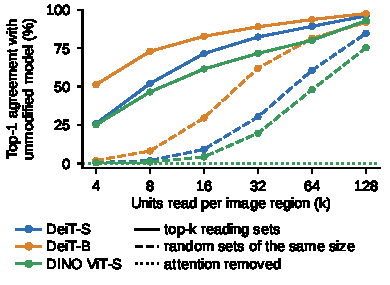
\includegraphics[width=3.25in]{execution_k_sweep}
\captionof{figure}{Top-1 agreement on 5,000 ImageNet images with region-selected top-$k$ units (solid), random units (dashed) or attention removed (dotted). Stored 95\% intervals are at most $\pm1.5$ percentage points. Dotted curves use crop ratio 0.875 for all models; other curves use each checkpoint's main preprocessing.}
\label{fig:app-ksweep}
\end{minipage}\end{center}

\paragraph{Diagnostics per layer.} Distance from the centre explained 82--98\% of mean-map variance at layers 9--12. Before registration, we also measured raw value lengths on 11,919 ImageNet-S images (crop ratio 0.875; main DeiT runs: 0.9). Within each eligible image and head we divided the mean raw value length of high-norm patches by the median for ordinary patches. Averaging first within layers, then equally over layers 9--12, gave 0.29 for DeiT-S and 0.23 for DeiT-B. Only images containing high-norm patches contribute. The block-input norm defines those patches before LayerNorm; raw value length is measured after LayerNorm and value projection.

\paragraph{Recovery at the last layer.} In the supervised models, single-layer received attention is worse at layer 12 than at the best of layers 8--11 (ClickMe values in Table~\ref{tab:app-diag}). Applied to layer 12, value weighting recovers 62\% and 33\% of this drop on enrichment (DeiT-S, DeiT-B), 31\% and 45\% on ClickMe alignment, and 8\% and 29\% on deletion. The other two corrections make layer 12 worse.

\begin{table}[!htbp]
\caption{Per-layer diagnostics (Fig.~\ref{fig:diag}a--c: ImageNet-S for the mean-map and high-norm shares; 2,000 held-out images for probe accuracy) and uncorrected ClickMe alignment (last three columns). S, B, D: DeiT-S, DeiT-B, DINO ViT-S; probe chance: 0.5\%. Values are rounded; DINO layers 9--12 have exactly zero high-norm attention on this dataset.}
\label{tab:app-diag}
\centering
% Generated from results/diagnose.csv.
\footnotesize
\setlength{\tabcolsep}{2.6pt}
\begin{tabular}{r >{\centering\arraybackslash}p{0.8cm} >{\centering\arraybackslash}p{0.8cm} >{\centering\arraybackslash}p{0.8cm} >{\centering\arraybackslash}p{0.8cm} >{\centering\arraybackslash}p{0.8cm} >{\centering\arraybackslash}p{0.8cm} >{\centering\arraybackslash}p{0.8cm} >{\centering\arraybackslash}p{0.8cm} >{\centering\arraybackslash}p{0.8cm} >{\centering\arraybackslash}p{1.05cm} >{\centering\arraybackslash}p{1.05cm} >{\centering\arraybackslash}p{1.05cm}}
\toprule
 & \multicolumn{3}{c}{\makecell{Specificity:\\mean-map share (\%)}} & \multicolumn{3}{c}{\makecell{Location:\\probe accuracy (\%)}} & \multicolumn{3}{c}{\makecell{Output magnitude:\\high-norm share (\%)}} & \multicolumn{3}{c}{\makecell{Map quality:\\ClickMe alignment}} \\
\cmidrule(lr){2-4}\cmidrule(lr){5-7}\cmidrule(lr){8-10}\cmidrule(lr){11-13}
Layer & S & B & D & S & B & D & S & B & D & S & B & D \\
\midrule
1 & 6.8 & 12.4 & 11.2 & 100.0 & 100.0 & 99.9 & 0.0 & 0.0 & 0.0 & $-$0.108 & $-$0.111 & $-$0.089 \\
2 & 21.2 & 14.0 & 7.4 & 100.0 & 100.0 & 100.0 & 0.0 & 0.0 & 0.0 & 0.007 & 0.041 & 0.064 \\
3 & 13.7 & 15.0 & 19.7 & 99.9 & 100.0 & 99.9 & 0.0 & 0.0 & 0.0 & 0.081 & 0.004 & 0.056 \\
4 & 6.9 & 7.5 & 14.6 & 99.0 & 100.0 & 99.8 & 0.0 & 0.0 & 0.0 & 0.132 & 0.110 & 0.140 \\
5 & 7.8 & 5.8 & 14.6 & 97.5 & 99.9 & 99.6 & 0.1 & 0.0 & 0.0 & 0.148 & 0.130 & 0.150 \\
6 & 5.2 & 6.2 & 11.9 & 85.3 & 99.5 & 98.9 & 2.6 & 0.0 & 0.0 & 0.136 & 0.151 & 0.167 \\
7 & 4.4 & 5.4 & 12.4 & 65.0 & 96.8 & 95.9 & 7.4 & 3.5 & 0.0 & 0.147 & 0.131 & 0.150 \\
8 & 4.2 & 5.4 & 6.6 & 43.9 & 91.8 & 85.6 & 9.3 & 12.9 & 0.0 & 0.149 & 0.118 & 0.170 \\
9 & 4.2 & 5.7 & 9.5 & 31.0 & 83.6 & 67.4 & 9.3 & 21.5 & 0.0 & 0.184 & 0.112 & 0.198 \\
10 & 4.3 & 5.5 & 15.2 & 23.1 & 66.8 & 50.5 & 9.1 & 28.1 & 0.0 & 0.171 & 0.139 & 0.207 \\
11 & 4.1 & 5.8 & 16.7 & 19.4 & 49.2 & 39.2 & 5.6 & 43.5 & 0.0 & 0.149 & 0.120 & 0.211 \\
12 & 3.3 & 5.0 & 13.6 & 18.1 & 31.8 & 35.7 & 7.2 & 22.2 & 0.0 & 0.098 & 0.023 & 0.179 \\
\bottomrule
\end{tabular}

\end{table}

\begin{table}[!tbp]
\caption{Paired differences, layers 9--12: mean, 95\% image-bootstrap interval and verdict (\textit{h}/\textit{c}/\textit{l}: higher/comparable/lower). Margins: 0.02 (enrichment/ClickMe), 0.05 (deletion); intervals unadjusted. Samples: App.~\ref{app:setup}. Top: each change (descriptive) and their combination (primary) versus received attention. Bottom: each change versus its matched control (primary). Registered negative controls are also discussed in App.~\ref{app:setup}.}
\label{tab:app-paired}
\centering
% Generated from results/correct_tests.csv; no statistical recalculation.
\footnotesize
\setlength{\tabcolsep}{4pt}
\renewcommand{\arraystretch}{1.08}
\begin{tabular}{lccc}
\toprule
Model & Same-ring enrichment & ClickMe alignment & Deletion score \\
\midrule
\multicolumn{4}{l}{\textit{Value weighting $-$ received attention}} \\
DeiT-S & 0.038 {\fontsize{8}{9}\selectfont [0.036, 0.039]}\,\textit{h} & 0.033 {\fontsize{8}{9}\selectfont [0.032, 0.034]}\,\textit{h} & 0.017 {\fontsize{8}{9}\selectfont [0.013, 0.021]}\,\textit{c} \\
DeiT-B & 0.065 {\fontsize{8}{9}\selectfont [0.063, 0.067]}\,\textit{h} & 0.058 {\fontsize{8}{9}\selectfont [0.056, 0.059]}\,\textit{h} & 0.029 {\fontsize{8}{9}\selectfont [0.024, 0.034]}\,\textit{c} \\
DINO ViT-S & $-$0.004 {\fontsize{8}{9}\selectfont [$-$0.004, $-$0.003]}\,\textit{c} & $-$0.001 {\fontsize{8}{9}\selectfont [$-$0.001, $-$0.001]}\,\textit{c} & 0.000 {\fontsize{8}{9}\selectfont [$-$0.003, 0.004]}\,\textit{c} \\
\addlinespace[2pt]
\multicolumn{4}{l}{\textit{Mean-map subtraction $-$ received attention}} \\
DeiT-S & $-$0.002 {\fontsize{8}{9}\selectfont [$-$0.003, $-$0.002]}\,\textit{c} & 0.009 {\fontsize{8}{9}\selectfont [0.008, 0.010]}\,\textit{c} & $-$0.028 {\fontsize{8}{9}\selectfont [$-$0.034, $-$0.023]}\,\textit{c} \\
DeiT-B & $-$0.003 {\fontsize{8}{9}\selectfont [$-$0.004, $-$0.003]}\,\textit{c} & $-$0.020 {\fontsize{8}{9}\selectfont [$-$0.021, $-$0.019]}\,\textit{l} & $-$0.025 {\fontsize{8}{9}\selectfont [$-$0.031, $-$0.019]}\,\textit{c} \\
DINO ViT-S & 0.002 {\fontsize{8}{9}\selectfont [0.001, 0.003]}\,\textit{c} & 0.044 {\fontsize{8}{9}\selectfont [0.040, 0.048]}\,\textit{h} & $-$0.052 {\fontsize{8}{9}\selectfont [$-$0.059, $-$0.044]}\,\textit{l} \\
\addlinespace[2pt]
\multicolumn{4}{l}{\textit{Probe relocation $-$ received attention}} \\
DeiT-S & $-$0.099 {\fontsize{8}{9}\selectfont [$-$0.101, $-$0.097]}\,\textit{l} & $-$0.073 {\fontsize{8}{9}\selectfont [$-$0.076, $-$0.069]}\,\textit{l} & $-$0.161 {\fontsize{8}{9}\selectfont [$-$0.171, $-$0.150]}\,\textit{l} \\
DeiT-B & $-$0.054 {\fontsize{8}{9}\selectfont [$-$0.055, $-$0.052]}\,\textit{l} & $-$0.057 {\fontsize{8}{9}\selectfont [$-$0.059, $-$0.055]}\,\textit{l} & $-$0.118 {\fontsize{8}{9}\selectfont [$-$0.127, $-$0.110]}\,\textit{l} \\
DINO ViT-S & $-$0.115 {\fontsize{8}{9}\selectfont [$-$0.117, $-$0.113]}\,\textit{l} & $-$0.064 {\fontsize{8}{9}\selectfont [$-$0.067, $-$0.062]}\,\textit{l} & $-$0.144 {\fontsize{8}{9}\selectfont [$-$0.153, $-$0.134]}\,\textit{l} \\
\addlinespace[2pt]
\multicolumn{4}{l}{\textit{All three corrections $-$ received attention}} \\
DeiT-S & $-$0.081 {\fontsize{8}{9}\selectfont [$-$0.083, $-$0.079]}\,\textit{l} & $-$0.034 {\fontsize{8}{9}\selectfont [$-$0.038, $-$0.030]}\,\textit{l} & $-$0.160 {\fontsize{8}{9}\selectfont [$-$0.171, $-$0.149]}\,\textit{l} \\
DeiT-B & $-$0.001 {\fontsize{8}{9}\selectfont [$-$0.003, 0.001]}\,\textit{c} & 0.030 {\fontsize{8}{9}\selectfont [0.027, 0.032]}\,\textit{h} & $-$0.084 {\fontsize{8}{9}\selectfont [$-$0.093, $-$0.076]}\,\textit{l} \\
DINO ViT-S & $-$0.111 {\fontsize{8}{9}\selectfont [$-$0.114, $-$0.109]}\,\textit{l} & $-$0.031 {\fontsize{8}{9}\selectfont [$-$0.035, $-$0.027]}\,\textit{l} & $-$0.195 {\fontsize{8}{9}\selectfont [$-$0.205, $-$0.184]}\,\textit{l} \\
\midrule
\multicolumn{4}{l}{\textit{Value weighting $-$ zero high-norm scores (its control)}} \\
DeiT-S & 0.026 {\fontsize{8}{9}\selectfont [0.025, 0.027]}\,\textit{h} & 0.022 {\fontsize{8}{9}\selectfont [0.021, 0.023]}\,\textit{h} & 0.012 {\fontsize{8}{9}\selectfont [0.008, 0.016]}\,\textit{c} \\
DeiT-B & 0.025 {\fontsize{8}{9}\selectfont [0.024, 0.026]}\,\textit{h} & 0.017 {\fontsize{8}{9}\selectfont [0.016, 0.018]}\,\textit{c} & 0.013 {\fontsize{8}{9}\selectfont [0.008, 0.018]}\,\textit{c} \\
DINO ViT-S & $-$0.004 {\fontsize{8}{9}\selectfont [$-$0.004, $-$0.003]}\,\textit{c} & $-$0.001 {\fontsize{8}{9}\selectfont [$-$0.001, $-$0.001]}\,\textit{c} & 0.000 {\fontsize{8}{9}\selectfont [$-$0.003, 0.004]}\,\textit{c} \\
\addlinespace[2pt]
\multicolumn{4}{l}{\textit{Mean-map subtraction $-$ centre-Gaussian subtraction (its control)}} \\
DeiT-S & 0.005 {\fontsize{8}{9}\selectfont [0.004, 0.005]}\,\textit{c} & $-$0.003 {\fontsize{8}{9}\selectfont [$-$0.005, $-$0.001]}\,\textit{c} & 0.040 {\fontsize{8}{9}\selectfont [0.034, 0.047]}\,\textit{c} \\
DeiT-B & 0.022 {\fontsize{8}{9}\selectfont [0.021, 0.023]}\,\textit{h} & 0.025 {\fontsize{8}{9}\selectfont [0.020, 0.030]}\,\textit{h} & 0.120 {\fontsize{8}{9}\selectfont [0.109, 0.130]}\,\textit{h} \\
DINO ViT-S & 0.001 {\fontsize{8}{9}\selectfont [0.001, 0.002]}\,\textit{c} & $-$0.001 {\fontsize{8}{9}\selectfont [$-$0.001, 0.000]}\,\textit{c} & 0.001 {\fontsize{8}{9}\selectfont [$-$0.003, 0.005]}\,\textit{c} \\
\addlinespace[2pt]
\multicolumn{4}{l}{\textit{Probe relocation $-$ matched blur (its control)}} \\
DeiT-S & $-$0.054 {\fontsize{8}{9}\selectfont [$-$0.056, $-$0.051]}\,\textit{l} & $-$0.068 {\fontsize{8}{9}\selectfont [$-$0.073, $-$0.064]}\,\textit{l} & $-$0.105 {\fontsize{8}{9}\selectfont [$-$0.116, $-$0.095]}\,\textit{l} \\
DeiT-B & 0.035 {\fontsize{8}{9}\selectfont [0.034, 0.036]}\,\textit{h} & $-$0.018 {\fontsize{8}{9}\selectfont [$-$0.020, $-$0.015]}\,\textit{c} & $-$0.047 {\fontsize{8}{9}\selectfont [$-$0.055, $-$0.037]}\,\textit{c} \\
DINO ViT-S & $-$0.105 {\fontsize{8}{9}\selectfont [$-$0.107, $-$0.102]}\,\textit{l} & $-$0.083 {\fontsize{8}{9}\selectfont [$-$0.085, $-$0.080]}\,\textit{l} & $-$0.146 {\fontsize{8}{9}\selectfont [$-$0.155, $-$0.137]}\,\textit{l} \\
\bottomrule
\end{tabular}

\end{table}

\begin{samepage}\paragraph{Differences behind Table~\ref{tab:main}.} Table~\ref{tab:app-paired} gives the paired differences with their intervals. The values in Table~\ref{tab:main} have 95\% intervals of at most $\pm0.005$ on enrichment and ClickMe alignment and $\pm0.012$ on deletion. The model-side differences from DeiT-S received attention are $+0.012$ [$0.011$, $0.013$] on enrichment, $+0.013$ [$0.012$, $0.013$] on ClickMe and $0.000$ [$-0.005$, $0.004$] on deletion for the test-time register, and $-0.040$ [$-0.042$, $-0.039$] and $-0.042$ [$-0.044$, $-0.040$] on the first two for top-$k$ training. The paired MiTA enrichment contrast uses 12,118 images valid for both models.\par\end{samepage}

\paragraph{What drives the value-weighting gain?} Value weighting reduces the relative weight of attention attached to small transformed-value vectors. One consequence was registered (P4a); additional checks were post hoc. \emph{No practically meaningful gain in DINO (P4a).} In DINO ViT-S, with zero high-norm attention at layers 9--12 on ImageNet-S, every difference from received attention is at most 0.004 in size (Table~\ref{tab:app-paired}). \emph{High-norm attention and alignment gain (post hoc).} Across images, gains have a weak positive association with the share of received attention on high-norm tokens: Spearman $+0.075$ [$0.057$, $0.092$] and $+0.132$ [$0.113$, $0.150$] on enrichment (DeiT-S, DeiT-B), $+0.045$ [$0.032$, $0.060$] and $+0.158$ [$0.143$, $0.173$] on ClickMe. \emph{Assigned versus shuffled weights (post hoc).} Against the same weights shuffled among the patches of each head, value weighting is higher in all four supervised cells: $+0.038$ [$0.037$, $0.040$] and $+0.073$ [$0.071$, $0.076$] on enrichment, $+0.035$ [$0.035$, $0.036$] and $+0.067$ [$0.065$, $0.068$] on ClickMe. The shuffle control averages seeds 0--4 within each image before bootstrap resampling. Projected minus raw value weighting ranged from $-0.0104$ to $-0.0004$ across the six model--alignment comparisons. None reached the 0.02 margin; the study did not test equivalence. Value weighting aggregates per-head terms related to \citet{kobayashi2020} and shares a norm-weighted component with \citet{zhu2024}; their full analyses and aggregation differ.

% =====================================================================================================
\subsection{Parameter-randomisation sanity check}
\label{app:sanity}

The original study included a model-parameter randomisation check~\citep{adebayo2018} on 1,000 fixed-seed ImageNet-S images. Parameters were cumulatively re-initialised from the classifier and final norm through blocks 12--1 to the patch/position embeddings and CLS token. The trained model's probes and mean maps remained fixed. Received attention and its corrections are class-agnostic and therefore do not depend on classifier parameters alone. Table~\ref{tab:sanity} reports the stored median per-image Spearman correlations between trained and fully randomised maps, with layers 9--12 summed. All five readings meet the registered median $<0.5$ criterion; the model-independent centre Gaussian fails as designed. This is a necessary sensitivity check, not proof of prediction faithfulness.

\begin{table}[!htbp]
\caption{Stored model-randomisation results: median map correlation after full randomisation. The five readings pass the registered $<0.5$ criterion in every model.}
\label{tab:sanity}
\centering\small
% Historical registered randomisation results from results/sanity.csv.
\begin{tabular}{@{}lrrr@{}}
\toprule
Reading & DeiT-S & DeiT-B & DINO ViT-S\\
\midrule
Received attention & $-$0.033 & 0.055 & 0.071 \\
Mean-map subtraction & 0.187 & 0.366 & 0.100 \\
Probe relocation & 0.063 & 0.004 & $-$0.002 \\
Value weighting & $-$0.064 & 0.070 & 0.114 \\
All three corrections & 0.069 & 0.078 & 0.025 \\
\midrule
Centre Gaussian & 1.000 & 1.000 & 1.000 \\
\bottomrule
\end{tabular}

\end{table}

\subsection{Alternative deletion endpoints}
\paragraph{Deletion endpoints.} For each image and method, trapezoidal integration uses the original removal budgets, divided by 196. The probability endpoint integrates the probability of the original top-1 class under least-important-first removal minus most-important-first removal. The KL endpoint uses the reverse difference in divergence from the original prediction, so that larger scores again indicate greater separation. For both endpoints the paired curve difference is zero at budget zero. These measures have no registered practical margin. An advantage in integrated area can reverse at a small removal budget; see the \href{https://github.com/hhuang999/vit-fastweight-lens/blob/main/docs/figures/deletion_curves.pdf}{budget-wise curves and intervals}.

\begin{center}\begin{minipage}{\linewidth}
\captionof{table}{Exploratory endpoint differences (value weighting minus comparator). Probability and KL columns give the mean paired area and 95\% image-bootstrap interval over the fixed 2,000-image deletion subset. ClickMe uses the original 17,408 images with batch-bootstrap intervals. KL has units of nats times fraction removed.}
\centering\footnotesize\setlength{\tabcolsep}{3pt}
\begin{tabular}{@{}llrrr@{}}
\toprule
Model & Comparator & Probability area & KL area & ClickMe \\
\midrule
DeiT-S & Received attention & 0.014 [0.012, 0.015] & 0.058 [0.050, 0.066] & 0.033 [0.032, 0.034] \\
DeiT-S & Zero high-norm & 0.010 [0.009, 0.012] & 0.041 [0.033, 0.049] & 0.022 [0.021, 0.023] \\
DeiT-B & Received attention & 0.022 [0.020, 0.024] & 0.107 [0.096, 0.118] & 0.058 [0.056, 0.059] \\
DeiT-B & Zero high-norm & 0.010 [0.008, 0.012] & 0.048 [0.038, 0.058] & 0.017 [0.016, 0.018] \\
DINO & Received attention & 0.000 [$-$0.001, 0.002] & $-$0.003 [$-$0.009, 0.003] & $-$0.001 [$-$0.001, $-$0.001] \\
DINO & Zero high-norm & 0.000 [$-$0.001, 0.002] & $-$0.003 [$-$0.009, 0.003] & $-$0.001 [$-$0.001, $-$0.001] \\
\bottomrule
\end{tabular}

\end{minipage}\end{center}
\subsection{Object geometry and the enrichment scale}
For an image with $M$ valid patches and $k>0$ foreground patches, let ring $r$ contain $m_r$ valid patches of which $f_r$ are foreground. Selecting a patch in this ring contributes $(y-f_r/m_r)/k$ to enrichment, where $y$ is its foreground indicator. Foreground contributions are nonnegative and background contributions are nonpositive. Selecting all $k$ foreground patches therefore attains the maximum
\[
 E_{\max}=1-\frac{1}{k}\sum_{r:m_r>0}\frac{f_r^2}{m_r}\ \le\ 1-\frac{k}{M}.
\]
The inequality follows by Cauchy--Schwarz. It bounds the score itself. The gain over received attention also depends on its starting score. A large raw improvement for small objects can thus reflect properties of both the map and the metric.
\paragraph{Area and centroid displacement.} Object area is the share of valid patch slots labelled foreground. Centroid displacement is the distance from their centroid to the grid centre, in patches. For each checkpoint we computed the empirical quartiles on its finite-geometry images, assigning ties to the lower bin. The DeiT area cut points were 0.158, 0.342 and 0.571. DINO's different crop produced different masks. Intervals use 2,000 paired image resamples from the same supplementary run. In DeiT-S and DeiT-B the largest-minus-smallest area quartile differences in the value weighting gain were $-0.090$ and $-0.157$ for enrichment. Comparing the most off-centre with the most central quartile instead gave $+0.057$ and $+0.095$. Area and centroid displacement covary. Among the smallest objects the latter differences were $+0.041$ [0.028, 0.053] and $+0.047$ [0.028, 0.066]. Some joint bins are small and these are observational contrasts.

\paragraph{Metric sensitivity.} After seeing the enrichment gradients we examined patch AUROC under the same quartile cut points. AUROC is the probability that a foreground patch outranks a background patch, counting ties as one half. In the supervised models the gain in AUROC persists across area quartiles (Table~\ref{tab:geometry}). AUROC does not condition on radius, so this comparison changes spatial adjustment as well as how foreground patches are selected. Relative to received attention, value weighting changes AUROC by $+0.028$, $+0.046$ and $-0.005$ for DeiT-S, DeiT-B and DINO.

\begin{center}\begin{minipage}{\linewidth}
\captionof{table}{Mean value weighting minus received attention by foreground-area quartile on ImageNet-S. Q1 contains the smallest objects. Both metrics use the same within-model cut points. AUROC excludes all-foreground crops.}
\label{tab:geometry}\centering\small\begin{tabular}{@{}llrrrr@{}}
\toprule
Metric & Model & Q1 & Q2 & Q3 & Q4 \\
\midrule
Enrichment & DeiT-S & 0.092 & 0.041 & 0.013 & 0.002 \\
Enrichment & DeiT-B & 0.165 & 0.060 & 0.026 & 0.008 \\
Enrichment & DINO & $-$0.003 & $-$0.004 & $-$0.005 & $-$0.003 \\
AUROC & DeiT-S & 0.024 & 0.030 & 0.031 & 0.026 \\
AUROC & DeiT-B & 0.042 & 0.048 & 0.048 & 0.046 \\
AUROC & DINO & 0.000 & $-$0.002 & $-$0.006 & $-$0.013 \\
\bottomrule
\end{tabular}

\end{minipage}\end{center}
\clearpage
\section{Tests of spatial relocation}
\label{app:reloc}

Relocation lowered all nine deep-layer scores relative to received attention (Table~\ref{tab:main}). Two planned comparisons narrow the problem. Early relocation remains comparable under the registered rule (P4b): at layers 1--4 it changes enrichment and ClickMe alignment by at most 0.004 in every model. In DeiT-S and DINO ViT-S, it also scored below blur matched for mean squared displacement (Table~\ref{tab:app-paired}). The rest of this section is post hoc: Table~\ref{tab:app-reloc} lists four explanations that we tested after seeing this result; none meets its specified criterion. Only 2--29\% of the probe's error mass lay more than three patches from the true slot. Replacing the linear probe with the tested MLP did not restore alignment. The probe targets index decodability rather than input-content provenance; whether this mismatch explains the failed relocation remains untested (Section~\ref{sec:method}).

\begin{table}[!htbp]
\caption{Four explanations for probe-relocation failure (post hoc). Model order: DeiT-S, DeiT-B, DINO ViT-S. Cells are the two centre-controlled metrics in the three models; criteria and probe settings are defined in this section.}
\label{tab:app-reloc}
\centering
% Four candidate explanations for the failure of probe relocation, each with its test and result.
% Authored summary of results/c2_analysis/{errors,mean_prediction}.csv and
% results/supplementary/{mlp_probe,globalisation}.csv; no number is computed here.
\footnotesize
\setlength{\tabcolsep}{4pt}
\renewcommand{\arraystretch}{1.0}
\begin{tabular}{@{}>{\raggedright\arraybackslash}p{2.9cm}>{\raggedright\arraybackslash}p{4.7cm}>{\raggedright\arraybackslash}p{5.75cm}@{}}
\toprule
Explanation & Test (layers 9--12 unless stated) & Result \\
\midrule
The probe sends score to distant patches & Share of the probe's error mass more than three patches from the true patch & Small: 2--29\% across models and layers. At layer 12, 45\%, 66\% and 81\% of the probability lies in the $3{\times}3$ neighbourhood of the true patch \\
The probe has a fixed position preference & Peak of the probe's mean prediction relative to uniform; its correlation with the mean map & Close to uniform (peak 1.1--1.3 times the uniform value); at most weakly related to the mean map \\
The linear probe is too weak & Two-layer MLP probe in place of the linear one & Layer-12 accuracy rises by only 1.8, 3.8 and 6.7 points; relocation is still lower than received attention in all six cells \\
Global tokens are harder to place & Probe accuracy and entropy against a token's similarity to the image's mean token (layers 10--12) & No consistent relation; accuracy falls with globality only in DeiT-B \\
\bottomrule
\end{tabular}

\end{table}

% =====================================================================================================
\paragraph{Probe capacity and explanatory criteria.} The tested MLP has a 1,024-unit hidden layer, GELU and a 196-way output. It uses the linear probe's optimiser, epochs, minibatches and standardisation, trained on 1,800 of the original probe-training images with 200 for best-validation-epoch selection; the original 2,000 test images remain separate. After observing the original relocation result, we specified the following criteria before running these follow-up tests: error mass beyond three patches greater than 0.5 at every deep model/layer; fixed preference peak at least twice uniform and mean-map correlation at least 0.5 (with positive lower interval bound) in every deep model/layer; MLP layer-12 accuracy gain above 10 percentage points in some model, with relocation rescued if it is not lower in at least 4/6 alignment comparisons. None of these criteria was met. This MLP comparison leaves other probe designs and calibration errors open.

\paragraph{Globality analysis.} Excluding high-norm tokens, globality is a token's cosine similarity to the mean of the other retained tokens in the image. Tokens are split into five equal-size rank groups. We relate the group rank to index accuracy and probe entropy, overall and within four equal-count radial groups, at layers 10--12. After observing the original relocation result, we set a follow-up criterion requiring negative accuracy and positive entropy associations (overall intervals and within-ring means) in at least two models. No consistent relationship meets this criterion.

\clearpage
\section{Example maps}
\label{app:gallery}

We drew 24 ClickMe images at random with a fixed seed. Fig.~\ref{fig:app-gallery-first} shows the two with the smallest ClickMe index, and Fig.~\ref{fig:app-gallery} the next four. Received attention and value weighting look much alike, while probe relocation spreads the score over many more patches. Because each panel has its own colour scale, use Table~\ref{tab:main} to assess changes in patch ranking across images.

\begin{center}\begin{minipage}{\linewidth}
\centering
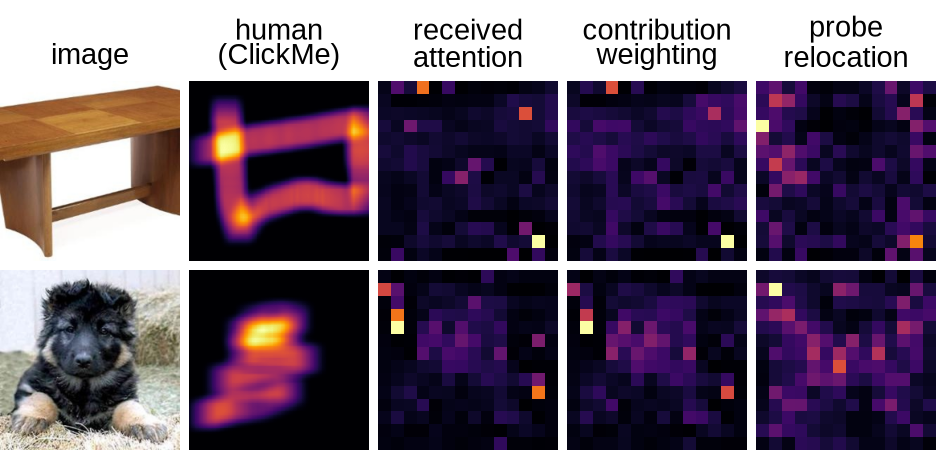
\includegraphics[width=4.7in]{example_maps}
\captionof{figure}{The first two fixed-seed examples, DeiT-S, layers 9--12. Colours show scores min--max normalised within each map; amplitudes are not comparable across panels. These images were not selected for correction gain.}
\label{fig:app-gallery-first}
\end{minipage}\end{center}

\begin{center}\begin{minipage}{\linewidth}
\centering
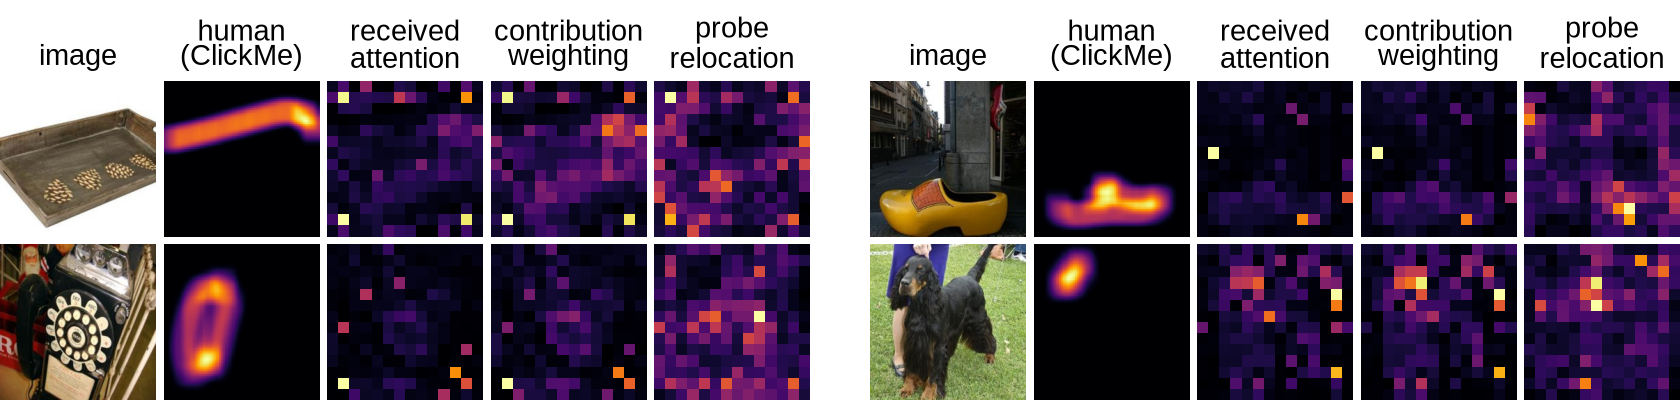
\includegraphics[width=5.5in]{example_maps_more}
\captionof{figure}{DeiT-S on four further ClickMe images, layers 9--12; colours are normalised within each map and do not compare amplitudes across panels.}
\label{fig:app-gallery}
\end{minipage}\end{center}

% =====================================================================================================
\clearpage
\section{Details of the two exploratory tests}\label{app:explore}
\subsection{Independent pet-image controls}
We selected the first 384 Oxford test images in fixed filename-hash order. We resized the short side to 248 pixels and centre-cropped to 224, using bicubic interpolation for images and nearest-neighbour for trimaps. We ignored boundary pixels and excluded patches with no valid pixels. A patch was foreground if at least half its valid pixels were foreground. One crop contained only foreground. Adjacent images in hash order exchanged length ranks, preserving each recipient's lengths within each layer and head. Within-ring shuffles used the same permutation across heads for a given image and layer. The reverse control keeps projected lengths at their own patches. Within each image, layer and head it replaces received attention at every patch with the same mean over the 196 patch slots. This preserves each head's total patch attention but removes its spatial variation.

We evaluated all seven readouts on the same 383 eligible crops. Table~\ref{tab:pets} reports paired differences in the primary endpoint, same-ring enrichment; the table below gives corresponding differences in AUROC. Both use 95\% percentile intervals from 10,000 paired image-bootstrap draws (seed 2026), without a practical margin. A follow-up sensitivity check resampled the 192 donor pairs, weighting by the number of eligible images in each draw. Value weighting minus donor-rank gives 0.0223 [0.0187, 0.0261] in this check.
\begin{center}\begin{minipage}{\linewidth}
\captionof{table}{All seven spatial readouts on the same 383 pet crops. Each AUROC difference subtracts the AUROC of value weighting at the original positions. Mean attention preserves each head's total patch attention; net output sums head vectors before taking each query--source magnitude, then pools queries.}
\centering\small\setlength{\tabcolsep}{4pt}\begin{tabular}{@{}lrrr@{}}
\toprule
Reading & AUROC & $\Delta$AUROC [95\% CI] & Enrichment \\
\midrule
Received attention & 0.788 & $-$0.028 [$-$0.031, $-$0.026] & 0.141 \\
Value weighting (own lengths) & 0.817 & --- & 0.160 \\
Donor-image positions & 0.787 & $-$0.029 [$-$0.032, $-$0.026] & 0.137 \\
Within-ring permutation & 0.793 & $-$0.023 [$-$0.025, $-$0.021] & 0.138 \\
Own lengths, mean attention & 0.757 & $-$0.059 [$-$0.069, $-$0.049] & 0.120 \\
Unprojected value norm & 0.822 & 0.006 [0.005, 0.006] & 0.163 \\
Norm after summing heads & 0.809 & $-$0.008 [$-$0.009, $-$0.007] & 0.156 \\
\bottomrule
\end{tabular}

\end{minipage}\end{center}

\subsection{Last-block CLS value intervention}
A second fixed filename hash selected 128 of the 384 images independently of their scores. At block 12 we cached its input and the unmodified logits. For each patch $j$ we held the original CLS attention weights fixed and removed $t_j=\sum_h a^h_{\mathrm{CLS},j}z_j^h$ from the CLS attention output. The shared projection bias stayed in place. The remaining residual, token-wise MLP, final normalisation and classifier were evaluated for each modified CLS. If $m$ is the margin between the original highest and second-highest logits, the response was $|m_{-j}-m|$ for those same classes. This intervention concerns the contextualised token at that slot. Its input evidence can span multiple image regions.

We ranked the 196 patch responses within each image and compared each readout with that ranking using Spearman correlation. Independent full forward passes on four images at three patches each matched the cached logits to within $2.4\times10^{-6}$. Table~\ref{tab:cls} reports the paired query comparison.
\paragraph{Matched mask comparison.} After inspecting the classifier intervention we evaluated the saved layer-12 rankings on the same 128 images and masks. All 128 had eligible foreground and background patches. Table~\ref{tab:cls} reports the three outcomes with equal image weights. Keeping the CLS query fixed, moving from the sum of per-head magnitudes to net magnitude changed margin Spearman by $+0.0092$ [0.0069, 0.0116], enrichment by $+0.0037$ [0.0007, 0.0069] and AUROC by $+0.0002$ [$-0.0031$, 0.0033].

\subsection{Receiver comparison in DeiT-B}
\label{app:replication}
In DeiT-S, restricting the readout to CLS improved intervention ranking but reduced foreground AUROC. We tested whether both directions persisted in a second checkpoint. Before scoring DeiT-B, we specified both endpoints in \texttt{experiments/receiver\_review/}. We retained the same 128 pet images, preprocessing, block 12, five readouts, 196 interventions per image and bootstrap settings. All 128 crops contained both mask classes. This follow-up was exploratory relative to the main registration.

Independent full forward passes on four images at patches 0, 97 and 195 matched the cached logits and class margins to within $3\times10^{-6}$ (tolerance: 0.002).

\begin{center}\begin{minipage}{\linewidth}
\captionof{table}{All five layer-12 rankings on the same 128 images. Intervention $\rho$ measures agreement with CLS-path sensitivity; AUROC and enrichment compare the unmodified score maps with foreground masks.}
\centering\small\setlength{\tabcolsep}{4pt}\begin{tabular}{@{}llrrr@{}}
\toprule
Model & Readout & Intervention $\rho$ & Mask AUROC & Enrichment \\
\midrule
DeiT-S & All queries, attention & 0.696 & 0.754 & 0.117 \\
DeiT-S & Value weighting, all queries & 0.705 & 0.769 & 0.127 \\
DeiT-S & Value weighting, CLS only & 0.747 & 0.678 & 0.095 \\
DeiT-S & CLS, net vector & 0.756 & 0.678 & 0.098 \\
DeiT-S & CLS, attention & 0.730 & 0.666 & 0.081 \\
DeiT-B & All queries, attention & 0.589 & 0.649 & 0.051 \\
DeiT-B & Value weighting, all queries & 0.652 & 0.685 & 0.084 \\
DeiT-B & Value weighting, CLS only & 0.734 & 0.710 & 0.088 \\
DeiT-B & CLS, net vector & 0.751 & 0.719 & 0.096 \\
DeiT-B & CLS, attention & 0.675 & 0.676 & 0.062 \\
\bottomrule
\end{tabular}

\end{minipage}\end{center}

\begin{center}\begin{minipage}{\linewidth}
\captionof{table}{Paired effects of retaining only the CLS query in the sum of head magnitudes. Intervals are 95\% percentile intervals from 10,000 image-bootstrap draws, seed 2026; no registered practical margin is applied.}
\centering\small\begin{tabular}{@{}llr@{}}
\toprule
Model & Endpoint & CLS $-$ all queries [95\% CI] \\
\midrule
DeiT-S & Intervention $\rho$ & 0.041 [0.026, 0.057] \\
DeiT-S & Mask AUROC & $-$0.091 [$-$0.110, $-$0.074] \\
DeiT-S & Enrichment & $-$0.033 [$-$0.043, $-$0.023] \\
DeiT-B & Intervention $\rho$ & 0.082 [0.068, 0.096] \\
DeiT-B & Mask AUROC & 0.024 [0.013, 0.036] \\
DeiT-B & Enrichment & 0.005 [$-$0.005, 0.013] \\
\bottomrule
\end{tabular}

\end{minipage}\end{center}

Retaining cancellation between heads is another distinction: in DeiT-B, net magnitude versus summed head magnitudes changes intervention correlation by 0.017 [0.014, 0.020], AUROC by 0.009 [0.007, 0.011] and enrichment by 0.008 [0.005, 0.011].

\clearpage
\section{Key parts of the code}
\label{app:code}

Given the attention $a_{ij}^h$ and values $v_j^h$ of a layer, the readings are:

\begin{lstlisting}[language=Python]
def received_and_contribution(p, v, w_o, prefix=1):
    # p: [B,H,T,T]; v: [B,H,T,d]; w_o: [D,H,d]
    # T includes CLS; values include the value-projection bias.
    gram = torch.einsum('dhe,dhf->hef', w_o, w_o)
    length = torch.einsum('bhne,hef,bhnf->bhn', v, gram, v)
    length = length.clamp_min(0).sqrt()
    received = p.sum(2)  # sum over queries
    s = received.sum(1)[:, prefix:]
    c = (received * length).sum(1)[:, prefix:]
    return s, c

def relocate(s, probs):  # source j to predicted position p
    return torch.einsum('bj,bjp->bp', s, probs)
\end{lstlisting}

For the independent pet experiment, the following readouts vary the placement of lengths or remove spatial variation in received attention. Here $a$ has axes (image, head, query, patch), and $z$ contains each head's projected value vector. The implementation processes queries in chunks.
\begin{lstlisting}[language=Python]
# Own lengths versus the same lengths in a donor image's spatial order
length = z.norm(dim=-1)                         # [B, H, 196]
order = donor_length.argsort(dim=-1)
borrowed = torch.empty_like(length).scatter(-1, order, length.sort(-1).values)
received = a.sum(dim=2)
own_map = (received * length).sum(dim=1)
donor_map = (received * borrowed).sum(dim=1)
mean_attention_map = (received.mean(dim=-1, keepdim=True) * length).sum(dim=1)

# Magnitude after summing the head vectors for each query and patch
net_map = sum(torch.einsum('bhij,bhjd->bijd', chunk, z).norm(dim=-1).sum(1)
              for chunk in a.split(32, dim=2))
\end{lstlisting}

For the final-block intervention we hold the attention matrix fixed. This excerpt from the full-forward check removes one patch's term from the CLS query. The output projection retains its bias and the rest of the model runs normally.
\begin{lstlisting}[language=Python]
# p: [batch, head, query, source]; v: [batch, head, source, head_dim]
head_out = p @ v
head_out[:, :, 0, :] -= p[:, :, 0, source_patch + 1, None] * v[:, :, source_patch + 1, :]
full = head_out.transpose(1, 2).reshape(batch, tokens, -1)
return attn.proj_drop(attn.proj(attn.norm(full)))
\end{lstlisting}

\paragraph{AI Use Statement.} I set the direction of this project, chose a fast-weight perspective for studying ViT attention maps, and organized the paper around three assumptions about how these maps are interpreted. I used AI tools to help search the literature, design follow-up experiments, write code, run experiments, analyze results, and draft and revise the report.


\end{document}
